\section{Entwicklung und Durchführung der Modultests}

Um die Funktionalität und Zuverlässigkeit des Testprogramms zu gewährleisten, werden umfassende Modultests mit dem Testframework \glqq googletest\grqq\ durchgeführt. Für jede Klasse des 
Produktivcodes wird eine entsprechende Testklasse erstellt. Diese Testklassen erben von \glqq ::testing::Test\grqq\ und ermöglichen die Definition von Setup- und Teardown-Methoden, 
die jeweils vor und nach den Testfällen ausgeführt werden. Diese Methoden ermöglichen die Initialisierung und Bereinigung der Testumgebung. Somit wird eine konsistente Ausführung 
der Tests sicherstellt.

Ein spezielles Beispiel der Modultests ist der Test der Klasse \glqq ConfigurationHandler\grqq. In diesem Test werden verschiedene Muster-Konfigurationsdateien verwendet, um 
unterschiedliche Szenarien zu simulieren. Diese Dateien umfassen sowohl korrekte Konfigurationen als auch solche mit inkorrekten Datentypen oder Werten, die außerhalb des zulässigen 
Bereichs liegen. Listing \ref{lst:AuszugModultests} zeigt exemplarisch jeweils einen Modultest für diese Fälle:

\vspace{12pt}

\begin{lstlisting}[
    caption={Beispiel Modultests},
    label={lst:AuszugModultests},
    language=C++,
    style=myCPP
]
@\textcolor{FunctionsYellow}{TEST\_F}@(@\textcolor{ClassGreen}{ConfigurationHandlerTest}@, ValidConfigA)
{
  @\textcolor{black}{config}@.@\textcolor{black}{configFilename}@ = "../test/TEST1_configParameter.json";
  @\textcolor{FunctionsYellow}{EXPECT\_TRUE}@(@\textcolor{black}{config}@.@\textcolor{FunctionsYellow}{loadConfiguration}@(param));

  @\textcolor{FunctionsYellow}{EXPECT\_EQ}@(@\textcolor{black}{param}@.@\textcolor{black}{saveImages}@, true);
  @\textcolor{FunctionsYellow}{EXPECT\_EQ}@(@\textcolor{black}{param}@.@\textcolor{black}{numberImages}@, true);
  @\textcolor{FunctionsYellow}{EXPECT\_EQ}@(@\textcolor{black}{param}@.@\textcolor{black}{numberFolders}@, true);
  @\textcolor{FunctionsYellow}{EXPECT\_EQ}@(@\textcolor{black}{param}@.@\textcolor{black}{saveImagesInterval}@, 1);
  @\textcolor{FunctionsYellow}{EXPECT\_EQ}@(@\textcolor{black}{param}@.@\textcolor{black}{newFolderInterval}@, 10);
  @\textcolor{FunctionsYellow}{EXPECT\_EQ}@(@\textcolor{black}{param}@.@\textcolor{black}{createLog}@@\textcolor{black}{param.createLog}@, true);
  @\textcolor{FunctionsYellow}{EXPECT\_EQ}@(@\textcolor{black}{param}@.@\textcolor{black}{logLevel}@, 1);
  @\textcolor{FunctionsYellow}{EXPECT\_EQ}@(@\textcolor{black}{param}@.@\textcolor{black}{maxLogFiles}@, 3);
  @\textcolor{FunctionsYellow}{EXPECT\_EQ}@(@\textcolor{black}{param}@.@\textcolor{black}{maxLogSize}@, 5);
  @\textcolor{FunctionsYellow}{EXPECT\_EQ}@(@\textcolor{black}{param}@.@\textcolor{black}{createIssue}@, true);
  @\textcolor{FunctionsYellow}{EXPECT\_EQ}@(@\textcolor{black}{param}@.@\textcolor{black}{testID}@, "TestID");

  @\textcolor{FunctionsYellow}{EXPECT\_TRUE}@(@\textcolor{ClassGreen}{filesystem}@::@\textcolor{FunctionsYellow}{exists}@(@\textcolor{black}{param}@.@\textcolor{black}{outputPath}@));
  @\textcolor{FunctionsYellow}{EXPECT\_TRUE}@(@\textcolor{ClassGreen}{filesystem}@::@\textcolor{FunctionsYellow}{exists}@(@\textcolor{black}{param}@.@\textcolor{black}{imagesPath}@));
  @\textcolor{FunctionsYellow}{EXPECT\_TRUE}@(@\textcolor{ClassGreen}{filesystem}@::@\textcolor{FunctionsYellow}{exists}@(@\textcolor{black}{param}@.@\textcolor{black}{logsPath}@));

  @\textcolor{ClassGreen}{filesystem}@::@\textcolor{FunctionsYellow}{remove\_all}@(@\textcolor{black}{param}@.@\textcolor{black}{outputPath}@);
}

@\textcolor{FunctionsYellow}{TEST\_F}@(@\textcolor{ClassGreen}{ConfigurationHandlerTest}@, InvalidDatatypeBool)
{
  @\textcolor{black}{config}@.@\textcolor{black}{configFilename}@ = "../test/TEST3_configParameter.json";
  @\textcolor{FunctionsYellow}{EXPECT\_FALSE}@(@\textcolor{black}{config}@.@\textcolor{FunctionsYellow}{loadConfiguration}@(param));
}
\end{lstlisting}

Mithilfe der gültigen Muster-Konfigurationsdateien wird die korrekte Übernahme der in den Konfigurationsdateien festgelegten Werte in die entsprechenden Variablen überprüft. 
Ungültige Konfigurationsdateien dienen dazu, die Fähigkeit des Testprogramms zu validieren, Fehler zu erkennen und zu melden, um einen fehlerhaften Betrieb zu verhindern.

Ein Aspekt der Testimplementierung ist das Mocking externer Abhängigkeiten, um eine Isolation der Tests zu gewährleisten. Durch das Ersetzen realer Abhängigkeiten mit Mock-Objekten 
können Tests in einer kontrollierten Umgebung durchgeführt werden. Die Mock-Objekte simulieren dabei ein für den jeweiligen Modultest festgelegtes Verhalten der Abhängigkeiten.
Dies ist insbesondere für das Testen von Komponenten, die mit externen Systemen interagieren, von großer Bedeutung.

Für eine zuverlässige Überprüfung der Methode \glqq checkKeyboardHit\grqq\ (siehe Anhang: Seite \pageref{checkKeyboardHit} ab Zeile 618) ist es notwendig Systemaufrufe zu simulieren. Hierfür werden mittels Mocking verschiedene Systemaufrufe 
angepasst. Dies ermöglicht es, das Verhalten der Tastatureingabe ohne tatsächliche Benutzerinteraktion zu testen. Dafür sind Funktionen notwendig, die Standardbibliothekfunktionen
durch die gemockten Funktionen ersetzen.

Durch die Abdeckung jeder Klasse des Testprogramms mit Modultests wird eine hohe Sicherheit des Testablaufs gewährleistet. Aktuell existieren jedoch keine Modultests für die 
Callback-Funktion und die Hauptfunktion. Die Herausforderung besteht darin, dass durch die Nutzung des Impact Acquire \acs{SDK} zahlreiche Abhängigkeiten zu Klassen und Methoden 
bestehen, die potenziell gemockt werden müssen. Der Aufwand hierfür ist für ein solches Testprogramm unverhältnismäßig hoch. Dennoch decken die bestehenden Modultests viele 
potenzielle Fehlerquellen innerhalb der Callback-Funktion auf, beispielsweise durch Tests der Methoden zur Vorbereitung des Speicherns. Zusätzlich bietet das Impact Acquire \acs{SDK} 
selbst ein umfangreiches Fehlermanagement, das Fehlermeldungen an das Testprogramm weiterleitet.

Die Integration des Testframeworks mittels CMake erleichtert die Ausführung der Modultests erheblich. Nach dem Start der ausführbaren Testdatei wird im Terminal eine 
Übersicht der Tests sowie die Ergebnisse der einzelnen Modultests angezeigt:

\begin{figure}[htbp]
    \centering
      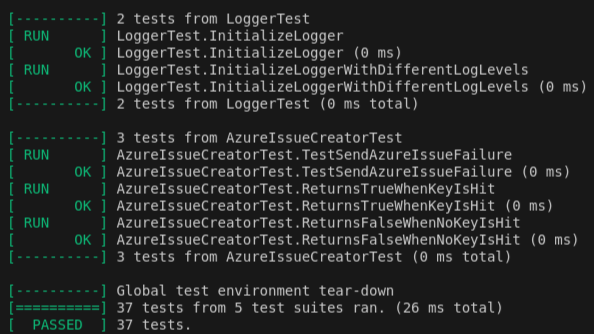
\includegraphics [width=0.75\textwidth]{ErgebnisModultests.png}
    \caption[Ergebnis Modultests]{Ergebnis Modultests (eigene Darstellung)}
    \label{fig:Modultests}
\end{figure}

Neben den Modultests wird das Testprogramm auch regelmäßig durch Verhaltenstests während der Entwicklungsphase überprüft. Somit werden Fehler frühzeitig identifiziert und behoben. 
Obwohl diese Tests die Testabdeckung temporär erhöhen, ist es wichtig zu erwähnen, dass sie nicht als Ersatz für eine systematische und dauerhafte Erweiterung der Testabdeckung durch 
Modultests dienen. Vielmehr ergänzen sie diese, indem sie zusätzliche Sicherheit bieten, dass das Programm auch unter realen Bedingungen zuverlässig funktioniert.